\scanpage{67}
\uline{Problèmes ouverts en théorie des Intersections.}

\uline{A. Grothendieck.}

\uline{Exposé $\overline{\underline{\mathrm{XIV}}}$}
\figure{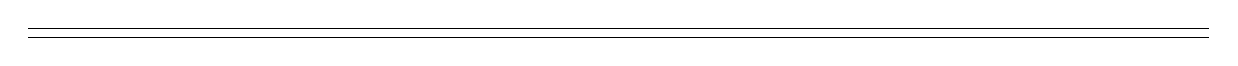
\begin{tikzpicture}\draw(0,0)--(15,0);\draw(0,.12)--(15,.12);\end{tikzpicture}}

\uline{Corrections à Faire après tirage}

\diagram{$\begin{array}{llll}
\text{p 14 -}&\text{ligne 59 -}&\text{est non nulle}&\text{(refaire NON)}\\[6pt]
\text{p 15 -}&\text{ligne 59 -}&\psi^3.&\text{(refaire }\psi\text{)}\\[6pt]
\text{p 2 -}&\text{ligne 17 -}&\overset{i}{\otimes}{}^L L.&\text{(refaire }\otimes\text{)}\\[6pt]
\text{p 19 -}&\text{ligne 3 -}&\text{7. clesses}&\text{(au lieu de cl\uuline{a}sses)}\\[6pt]
\text{p 17 -}&\text{ligne 12 -}&\text{\unsure{flêches|flâches}}&\text{(au lieu de fléches)}
\end{array}$}

\[
x\longmapsto\operatorname{Hom}(x,\unsure{\xi})\qquad\unsure{\xi}\text{ injectif}
\]
\diagram{\begin{tikzcd}
B^o\arrow[r,"F"]&\mathrm{Ab}_k\arrow[r,"\deleted{\unsure{*}}v"]&\mathrm{Ab}_k^o
\end{tikzcd}}
\diagram{\begin{tikzcd}B^o\arrow[r,dash]&\mathrm{Ab}_k\end{tikzcd}}
injectifs $\Longrightarrow$ injectifs de $\mathrm{Ab}_k^o$

i.e. des \uline{projectifs} de $\mathrm{Ab}_k$

\diagram{\begin{tikzcd}B^o\arrow[r]&\mathrm{Ab}\end{tikzcd}}
\deleted{$\unsure{\mathrm{Ab}_k}$}
\diagram{\begin{tikzcd}\mathcal M\arrow[r,"u"]&\mathcal M'\end{tikzcd}}
$u$ \uline{exact}, transforme injectifs en injectifs

\deleted{$\unsure{H^i}\quad C(F$}
$C^i$
\deleted{$\unsure{\mathrm{Ab}_k}$}
\[
\deleted{\unsure{t}}\ v(R\Gamma_{\unsure{\mathrm{Ab}_k}}(B,F))
\overset{?}{\simeq}R\Gamma(B,v\circ F)
\bigl(\simeq LH_\bullet(A^o,(v\circ F)^o)\bigr)
\]
$\Gamma(C^i)$
\figure{\begin{tikzpicture}
\draw(0,.1)..controls(2,0)and(3,-.2)..(4,-.1)..controls(4.8,0)and(4.2,.8)..(4.9,.95)..controls(6,1.2)and(8,1.3)..(9,1.15);
\end{tikzpicture}}
\[
LH_0(A,\int F)\mathbin{\text{---}}LH_\bullet(B,F)
\]
\[
F\in\widehat B_{\mathcal M}
\]
\diagram{\begin{tikzcd}\mathcal M\arrow[r]&\mathrm{Ab}_k\end{tikzcd}}
commute aux $\varinjlim$ et transforme projectifs en projectifs

\uline{ex.} $\mathcal M=M^{\unsure{\flat|h}}$,
\diagram{\begin{tikzcd}\mathrm{Ab}_k^o\arrow[r,"\text{contre}"]&\mathrm{Ab}_k\end{tikzcd}}
\mspage{66}
